\documentclass[tikz]{standalone}
\usepackage{pgfplots}
\pgfplotsset{compat=1.5.1}
\begin{document}
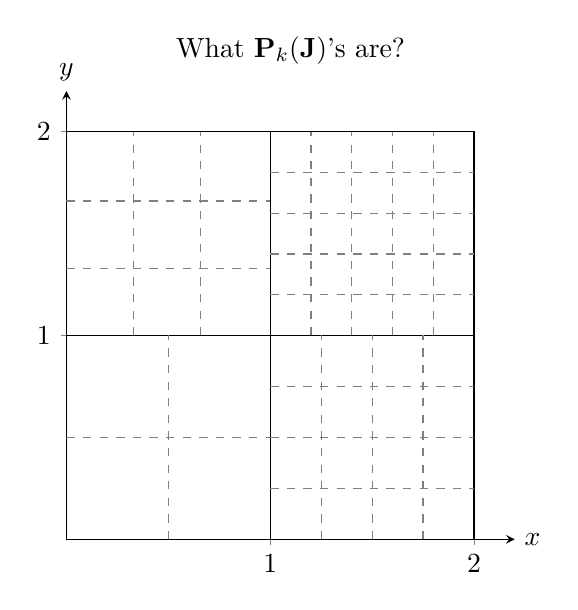
\begin{tikzpicture}
  \begin{axis}[
    title=What $\mathbf{P}_k (\mathbf{J})$'s are?,
    axis x line=middle, axis y line=middle,
    axis equal image=true,
    xlabel=$x$, ylabel=$y$,
    xlabel=$x$, xlabel style={at={(1,0)}, anchor=west},
    ylabel=$y$, ylabel style={at={(0,1)}, anchor=south},
    xmin=0, xmax=2.2, ymin=0, ymax=2.2,
    xtick={0,1,2}, ytick={0,1,2},
  ]
  \draw (axis cs:0,0) rectangle (axis cs:1,1);
  \draw (axis cs:1,0) rectangle (axis cs:2,1);
  \draw (axis cs:0,1) rectangle (axis cs:1,2);
  \draw (axis cs:1,1) rectangle (axis cs:2,2);

  % Vertical lines
  % First J
  \draw[dashed, color=gray] (axis cs:0.5,0) -- (axis cs:0.5,1);
  
  % Second J
  \draw[dashed, color=gray] (axis cs:0.33,1) -- (axis cs:0.33,2);
  \draw[dashed, color=gray] (axis cs:0.66,1) -- (axis cs:0.66,2);
  
  % Third J
  \draw[dashed, color=gray] (axis cs:1.25,0) -- (axis cs:1.25,1);
  \draw[dashed, color=gray] (axis cs:1.5,0) -- (axis cs:1.5,1);
  \draw[dashed, color=gray] (axis cs:1.75,0) -- (axis cs:1.75,1);
  
  % Fourth J
  \draw[dashed, color=gray] (axis cs:1.2,1) -- (axis cs:1.2,2);
  \draw[dashed, color=gray] (axis cs:1.4,1) -- (axis cs:1.4,2);
  \draw[dashed, color=gray] (axis cs:1.6,1) -- (axis cs:1.6,2);
  \draw[dashed, color=gray] (axis cs:1.8,1) -- (axis cs:1.8,2);

  % Horizontal lines
  % First J
  \draw[dashed, color=gray] (axis cs:0,0.5) -- (axis cs:1,0.5);
  
  % Second J
  \draw[dashed, color=gray] (axis cs:0,1.33) -- (axis cs:1,1.33);
  \draw[dashed, color=gray] (axis cs:0,1.66) -- (axis cs:1,1.66);
  
  % Third J
  \draw[dashed, color=gray] (axis cs:1,0.25) -- (axis cs:2,0.25);
  \draw[dashed, color=gray] (axis cs:1,0.5) -- (axis cs:2,0.5);
  \draw[dashed, color=gray] (axis cs:1,0.75) -- (axis cs:2,0.75);
  
  % Fourth J
  \draw[dashed, color=gray] (axis cs:1,1.2) -- (axis cs:2,1.2);
  \draw[dashed, color=gray] (axis cs:1,1.4) -- (axis cs:2,1.4);
  \draw[dashed, color=gray] (axis cs:1,1.6) -- (axis cs:2,1.6);
  \draw[dashed, color=gray] (axis cs:1,1.8) -- (axis cs:2,1.8);
  \end{axis}

\end{tikzpicture}
\end{document}
